\documentclass[a4paper,11pt,twocolumn]{article}
%\documentclass[dvips]{article}
\usepackage{graphicx}
\usepackage[spanish,activeacute]{babel}
\usepackage[margin=0.8in]{geometry}
\bibliographystyle{plain}
\usepackage{hyperref}
\usepackage{amssymb,amsmath}
%\usepackage{draftwatermark}
\usepackage{graphicx}
\usepackage{pseudocode}
\usepackage[normalem]{ulem}
%\SetWatermarkFontSize{40pt}
%\SetWatermarkScale{6}
\begin{document}

\setlength{\columnsep}{25pt}

\title{Midiendo la Performance de SPDY}
\author{Pablo Maximiliano Lulic}

\maketitle

\begin{abstract} 
Actualmente, la Web se sustenta con el est'andar \textsc{http}. Este protocolo tuvo su 'ultima versi'on en el a'no 1999. L'as p'aginas en ese entonces eran muy diferentes a las actuales, tanto en contenido como en cantidad de recursos. Google desarroll'o un protocolo en el a'no 2009 llamado \textsc{spdy}, cuyo prop'osito es mejorar la performance en la recuperaci'on de los recursos de la web. A pesar de su gran aceptaci'on, y de sentar las bases del pr'oximo \textsc{http 2.0}, hay ciertas cuestiones que todav'ia quedan por revisar. En este paper se propone evaluar, la performance de \textsc{spdy} desde dos enfoques diferentes, uno en ambientes espec'ificos y otro en la web.
\end{abstract}

\section{Introducci'on}

El protocolo \textsc{http} tuvo su primera versi'on en mayo de 1996, culminando en 1999 con el est'andar actual que es el \textsc{http}  1.1 \cite{rfcHTTP}. El mismo, es un protocolo sin estado, el servidor no mantiene informaci'on acerca de las diferentes peticiones que le llegan, lo que conlleva a que se necesite realizar una petici'on nueva por cada recurso que se necesite de un sitio web, incluso siendo del mismo dominio. Esto genera tr'afico innecesario entre petici'on y petici'on cuando el cliente necesita establecer una conexi'on nueva para obtener el recurso. Con \textsc{spdy} esta cuesti'on se ha resuelto y, junto con otras caracter'isticas que se ver'an mas adelante, se mejora la performance de la recuperaci'on de un sitio web.

Se realizar'an 2 experimentos, en ambos se evaluar'an los tiempos de carga de diferentes sitios (detallados m'as adelante), utilizando las siguientes medidas:

\begin{enumerate}
\item onContentLoad: Tiempo en el que el contenido del sitio se carga.
\item onLoad: Tiempo en el que es sitio se carga seg'un el navegador.
\item ToW (Time on Wire): Tiempo en el cable, medido desde el primer paquete que se env'ia al servidor hasta el 'ultimo.
\end{enumerate}

Se busca comparar la performance de \textsc{spdy} frente a \textsc{http} y \textsc{https}. El primer experimento se realizar'a en un ambiente controlado, emulando diferentes combinaciones de Ancho de Banda y Retardo, peticionando sitios descargados previamente. El segundo experimento se realizar'a en un ambiente real, recuperando sitios populares.

\section{La Web en la Actualidad}

En comparaci'on con lo que era la web en la 'epoca en la que se implement'o el protocolo \textsc{http}, hubo un marcado incremento en el tama'no y en la cantidad de recursos de un sitio web. Para Noviembre de 2013 \cite{httpArchive}, el tama'no promedio de un sitio era de 1614kb, en contraste con Noviembre de 2010 donde promediaba 702kb, hubo un incremento del 50\%. Estudios m'as recientes, indican que el crecimiento de una p'agina promedio es del 151\% (en un lapso de 3 a'nos) \cite{tammy} (ver Figura \ref{average}).

El crecimiento se produce con velocidad \cite{averageWebPage} y hay otras cuestiones relacionadas al tiempo de carga de una p'agina, no solo el ancho de banda \cite{moreBand}, sino tambi'en, el \textsc{rtt}\footnote{Tiempo que tarda un paquete de datos en ir desde el emisor al receptor y volver al emisor.}, como se puede ver en la Figura \ref{rttBelsche}, por ejemplo.

\begin{figure}[h!]
  	\centering
	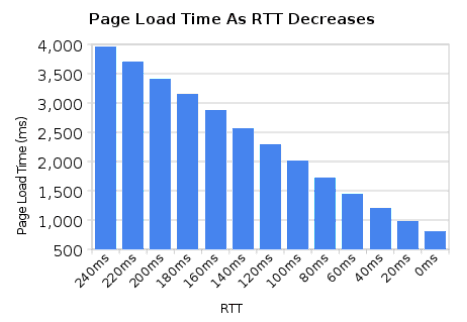
\includegraphics[scale=0.5]{belsche}
	\caption{\small Tiempo de carga de una p'agina mientras se var'ia el RTT, extra'ido de \cite{moreBand}}
	\label{rttBelsche}
\end{figure}

\section{SPDY}
\begin{figure}[h!]
  	\centering
	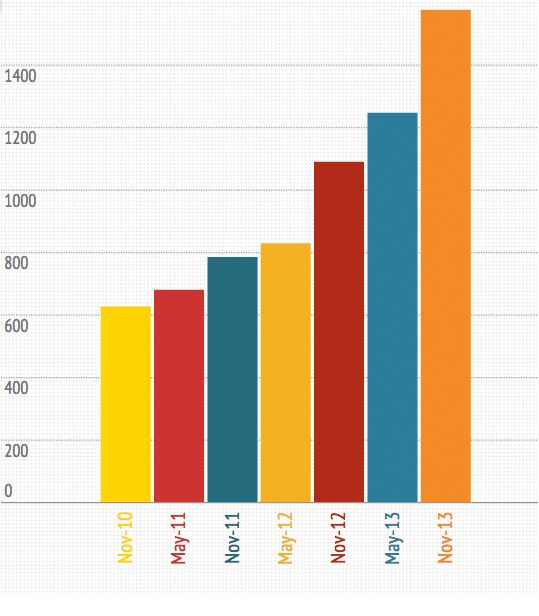
\includegraphics[scale=0.4]{151tammy}
	\caption{\small Crecimiento del tama'no de los sitios promedio, extra'ido de \cite{tammy}}
	\label{average}
\end{figure}
\textsc{spdy}\cite{SPDYWhitepaper} es un protocolo de la capa de aplicaci'on \cite{illustratedTCPIP} que funciona sobre SSL \cite{rfcSSL}, permite la transmisi'on de Streams\footnote{Flujo de Datos.} sobre una conexi'on normal de \textsc{tcp}, que es el Protocolo de Control de Transmisi'on de la Capa de Transporte \cite{illustratedTCPIP}. A continuaci'on se comentar'an las caracter'isticas del Protocolo (extra'idas de \cite{SPDYWhitepaper}):

\begin{enumerate}

\item Streams Multiplexados.

\item Priorizaci'on de Peticiones.

El Cliente puede peticionar tantos recursos como necesite del Servidor y asignarle prioridad a cada uno de ellos.

\item Compresi'on de los Headers \textsc{http} \cite{headersHTTP}.

Comprime los headers de petici'on y respuesta \textsc{http}.

\item Push

Permite al Servidor enviarle recursos al Cliente sin que este se lo pida.

\item Hint

Permite al Servidor ''sugerirle'' al Cliente que pida alg'un recurso espec'ifico.

\end{enumerate}

\section{Experimento 1}
\label{experimento1}
\subsection{Preparaci'on}

Se virtualizaron 3 m'aquinas utilizando VirtualBox \cite{virtualBox}, disponibles para su descarga en \cite{maqVirtuales}.
Se dise'no la topolog'ia de Red como se observa en la Figura \ref{diagramavms}.

\begin{figure*}[ht]
  \centering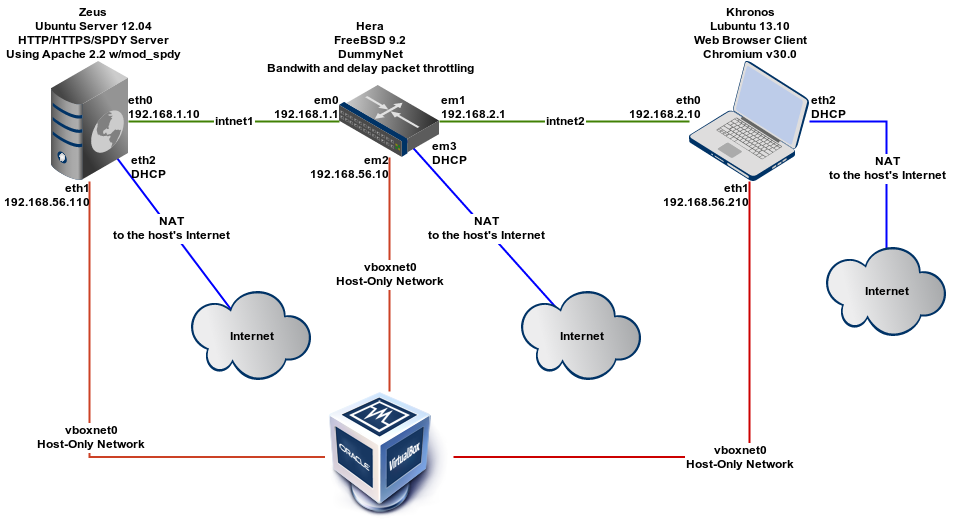
\includegraphics[scale=0.5]{diagramavms}
  \caption{Diagrama de Red del Entorno Virtual del Experimento 1}
  \label{diagramavms}
\end{figure*}

\begin{enumerate}
\item SERVIDOR

Se descargaron los sitios\footnote{Utilizando la opci'on ''Guardar como...'' de Google Chrome, que obtiene todos los recursos externos y los almacena en una carpeta.} y se configuraron los siguientes hosts virtuales en el Servidor:
\begin{enumerate}
\item www.amazon.com
\item www.bing.com
\item login.yahoo.com
\item www.world-flags.com \cite{flags}
\end{enumerate}

Cada sitio se brind'o utilizando el servidor Apache 2.2 \cite{apache}. En \textsc{http} plano con su configuraci'on por defecto, en \textsc{https} utilizando \emph{mod\_ssl} \cite{modSSL} con un certificado SSL autofirmado con Ubuntu \cite[Secci'on 4]{spdyGT}, para ofrecer \textsc{spdy}, se instal'o \emph{mod\_spdy} \cite{modSPDY}. Con el prop'osito de poder realizar un an'alisis de los paquetes que viajan luego de finalizado el experimento, se realiz'o la siguiente modificaci'on en la configuraci'on del SSL, que es el archivo \emph{''/etc/apache2/mods-enabled/ssl.conf''} \cite{siffSSL}.

\begin{quote}\small
\#   SSL Cipher Suite:

\#   List the ciphers that the client is permitted to negotiate.

\#   See the mod\_ssl documentation for a complete list.

\#   enable only secure ciphers:

\sout{\#SSLCipherSuite HIGH:MEDIUM:!ADH:!MD5}

SSLCipherSuite DES-CBC3-SHA
\end{quote}

\item PROXY

Utilizando la herramienta Dummynet \cite{dummynet} que viene instalada en la distribuci'on de FreeBSD, se utilizaron diferentes comandos \cite{ipfw} para filtrar el tr'afico en la red\footnote{Ancho de Banda y Retardo.} y simular diferentes entornos. Se habilit'o la Dummynet modificando el archivo \emph{''/etc/rc.conf''} con las siguientes l'ineas

\begin{quote}\small
firewall\_enable=''YES''

firewall\_type=''OPEN''

gateway\_enable=''YES''
\end{quote}

Se configur'o el siguiente flag:
\begin{quote}\small
sysctl net.inet.ip.forwarding=1
\end{quote}
Y por 'ultimo, para que la Dummynet inicie junto con el Kernel del FreeBSD se agreg'o la siguiente l'inea en el archivo \emph{''/bot/loader.conf''}
\begin{quote}\small
dummynet\_load=''YES''
\end{quote}
\item CLIENTE

Se instal'o \emph{NodeJS} \cite{nodeJS} y se descarg'o el software \emph{chrome-har-capturer} \cite{harCapt} de GitHub \cite{github}.
Se utiliz'o el navegador \emph{Chromium} Versi'on 30 que, a trav'ez de su API de depuraci'on remota \cite{debuggingChrome}, permite al \emph{chrome-har-capturer} interactuar con dicho navegador para poder navegar un sitio en particular y obtener un archivo \emph{.har}\footnote{Archivo con notaci'on JSON \cite{json} que contiene la traza del Navegador Web con el sitio}, que contiene los resultados de la interacci'on del navegador con el sitio. Por otro lado, fue utilizada la herramienta \emph{TShark}\cite{tshark} para poder capturar los paquetes que viajan en la red durante el experimento.

\end{enumerate} 

\subsection{Metodolog'ia}
 \label{exp1meto}
Con la idea de comparar los m'etodos \textsc{http}, \textsc{https} y \textsc{spdy} en diferentes ambientes simulados, se definieron los siguientes valores:

\vspace*{1\baselineskip}
\begin{tabular}{ l c r }
	Ancho de Banda (BW)  \\ \hline
  	100 Kbps \\
	256 Kbps \\
	512 Kbps \\
	1024 Kbps \\
	2048 Kbps \\
	5120 Kbps \\
	10240 Kbps \\
\end{tabular}
\vspace*{1\baselineskip}
\begin{tabular}{ l c r }
	Retraso (RTT) \\ \hline
  	10 ms \\
	50 ms \\
	100 ms \\
	200 ms \\
	250 ms \\
	500 ms \\
	\\
\end{tabular}

En el Proxy, se crea una \emph{tuber'ia}\footnote{Objeto intermediario donde se simulan diferentes entornos} de la siguiente manera.

\begin{quote}\small
ipfw add 1000 pipe 1 ip from any to any;
\end{quote}

Y los valores se van configurando autom'aticamente mediante el siguiente comando:

\begin{quote}\small
ipfw pipe 1 config bw 1000Kbp/s delay 100ms;
\end{quote}

Se combinaron todos los Anchos de Banda con todos los Retrasos para cada uno de los m'etodos por p'agina\footnote{Por ejemplo: 100Kbps de Ancho de Banda con 100ms de Retraso accediendo al host virtual de Amazon por \textsc{https} (https://www.amazon.com).}.

En el Servidor se activa \emph{mod\_spdy} seg'un es requerido, utilizando:

\begin{quote}\small
a2enmod spdy
\end{quote}

O desactivar:

\begin{quote}\small
a2dismod spdy
\end{quote}

Cuando el test no es para el m'etodo \textsc{spdy}, en el cliente  se desactiva tambi'en la utilizaci'on desde el Browser con el flag\footnote{http://peter.sh/experiments/chromium-command-line-switches/}:

\begin{quote}\small
--use-spdy=off
\end{quote}

El algoritmo\footnote{Disponible en \cite[exp1.sh]{spdy-tests}} fu'e el siguiente:

\begin{pseudocode}{experimento1}{ }
\FOR ancho\ de\ banda \in anchos\ de\ bandas \DO \\
	\BEGIN
	\FOR retardo \in retardos \DO \\
		\BEGIN
			configurar\ valores\ en\ el\ proxy \\
			\FOR metodo \in (http,https,spdy) \DO \\
				\BEGIN
					\IF metodo == spdy
					\THEN
						activar\ spdy\ en\ el\ servidor
					\ELSE
						desactivar\ spdy\ en\ el\ servidor\\
					\FOR sitio \in sitios \DO \\
					\BEGIN
						iniciar\ chrome\\
						iniciar\ captura\ con\ tshark\\
						ejecutar\ chrome-har-capturer\\
						cerrar\ chrome\\
						cerrar\ tshark
					\END
				\END
		\END
	\END
\end{pseudocode}

Se repiti'o el experimento 7 veces para poder promediar los resultados. La informaci'on obtenida (archivos .har y .pcap) se proces'o para obtener los tiempos basados en el \emph{.har} \cite{harSpec}, OnLoad y OnContentLoad y el basado en la captura de \emph{Tshark}, ToW. Estos resultados se almacenaron en una base de datos \emph{SQLite} \cite{SQLite} para su posterior an'alisis.

\subsection{Resultados}

En cuanto a las medidas seleccionadas para el experimento, se observ'o que, el valor del \emph{onContentLoad} presenta una diferencia notable con respecto a las otras 2 medidas (\emph{onLoad} y \emph{ToW}) cuando el sitio tiene mucho contenido (por ejemplo en los sitios de amazon y worldflags) (Ver Figura \ref{graf1}). En cambio cuando el sitio tiene escaso contenido (el caso de yahoo y bing), las medidas se encuentran m'as cercanas entre s'i (Ver Figura \ref{graf2}).

La medida \emph{onLoad}, es la que se encuentra m'as cerca del tiempo que percibe el usuario cuando el navegador que est'a utilizando, termina de renderizar el sitio en cuesti'on.

\begin{figure}[h!]
  	\centering
	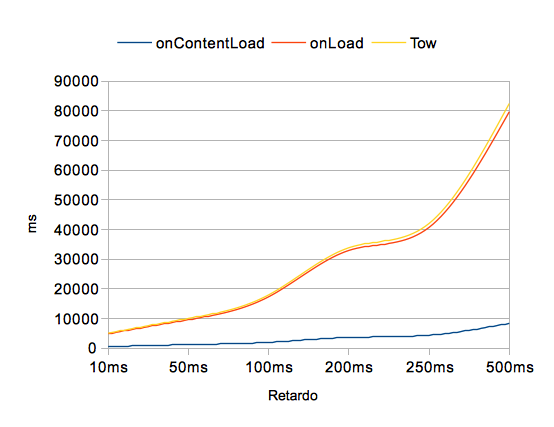
\includegraphics[scale=0.65]{exp1_1}
	\caption{\small www.worldflags.com - HTTPS - 1024Kbps}
	\label{graf1}
\end{figure}

\begin{figure}[h!]
  	\centering
	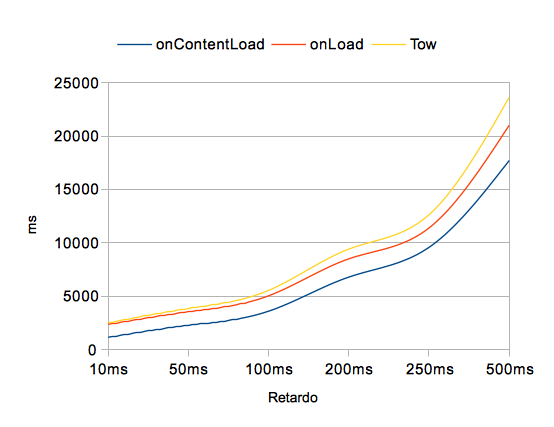
\includegraphics[scale=0.65]{exp1_2}
	\caption{\small www.bing.com - HTTPS - 1024Kbps}
	\label{graf2}
\end{figure}

Hay un caso en particular donde, la utilizaci'on de \textsc{spdy} mejora notablemente los tiempos de carga del sitios, lo que se observa con el caso de \emph{www.worldflags.com}, como se puede ver en la Figura \ref{graf3} y \ref{graf4}.

Este sitio est'a tomado de \cite{modspdyApache} y se puede ver online en \cite{flags}. Es el caso emblem'atico para el protocolo, ya que reune las caracter'isticas para que el funcionamiento de \textsc{spdy} sea el 'optimo. Es un sitio sencillo con 196 recursos (im'agenes) todas almacenadas en el mismo lugar, lo que aprovecha al m'aximo la utilizaci'on de los flujos de datos del protocolo; en contraposici'on con la cantidad de conexiones que se deben realizar (utilizando \textsc{http} o textsc{https}) con el servidor para traer tantos recursos.

\begin{figure}[h!]
  	\centering
	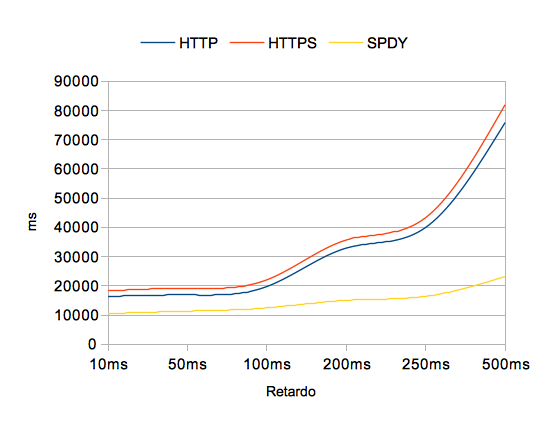
\includegraphics[scale=0.65]{exp1_3}
	\caption{\small www.worldflags.com - onLoad - 256Kbps}
	\label{graf3}
\end{figure}

\begin{figure}[h!]
  	\centering
	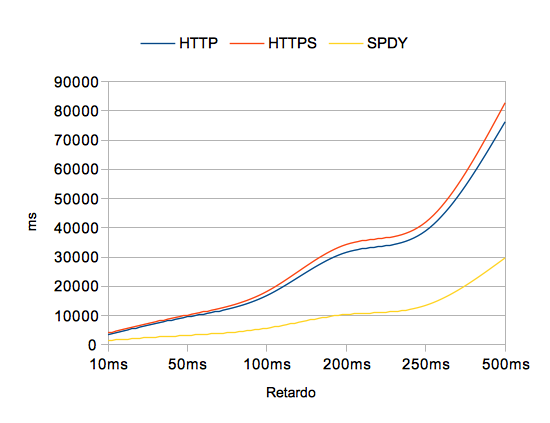
\includegraphics[scale=0.65]{exp1_4}
	\caption{\small www.worldflags.com - Tow - 10240Kbps}
	\label{graf4}
\end{figure}

Se observ'o el mismo comportamiento que plantea \emph{Mike Belshe} en \cite{moreBand}. Esto se puede ver en la Figura \ref{graf5}, en donde al incrementar el Ancho de Banda manteniendo el mismo retardo de 500ms, el tiempo de carga del sitio va formando una constante.

\begin{figure}[h!]
  	\centering
	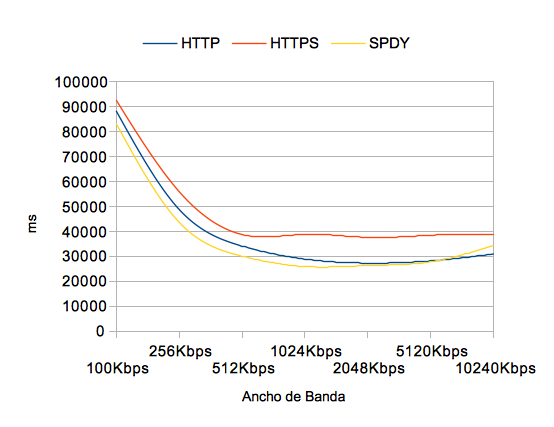
\includegraphics[scale=0.65]{exp1_5}
	\caption{\small login.yahoo.com - onLoad - 500ms}
	\label{graf5}
\end{figure}

El rendimiento de los protocolos cuando la velocidad es alta es similar, en cambio, cuando son sometidos a velocidades bajas, \textsc{spdy} mejora levemente su performance frente a los dem'as, tal como se ve en la Figura \ref{graf6}.

\begin{figure*}[ht]
  	\centering
	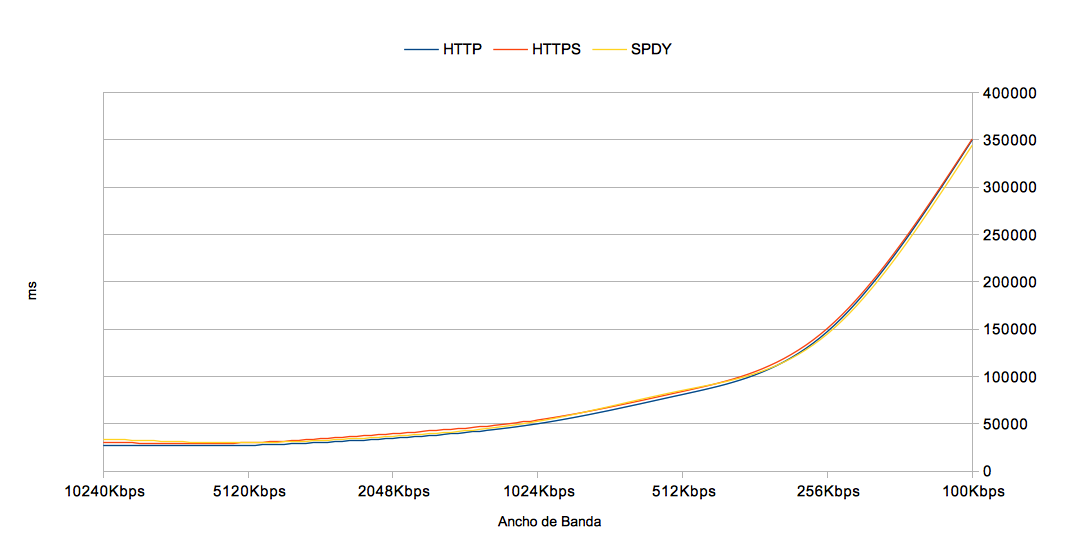
\includegraphics[scale=0.65]{exp1_6}
	\caption{\small www.amazon - onLoad - 250ms}
	\label{graf6}
\end{figure*}

\section{Experimento 2}
\label{experimento2}
\subsection{Preparaci'on}

Se configur'o un Cliente con las mismas caracter'isticas que las del Experimento 1 (ver secci'on \ref{experimento1}). Se seleccionaron los siguientes sitios, basados en el art'iculo \cite{effectSPDY}, adem'as se agregaron 2 sitios con contenido diferente al de la p'agina principal de 2 de los sitios testeados (blogspot-blogger y wordpress):
\begin{enumerate}
\item www.facebook.com
\item www.google.com
\item www.youtube.com
\item www.blogger.com
\item www.twitter.com
\item www.wordpress.com
\item www.imgur.com
\item www.youm7.com
\item consigueregalos.blogspot.com
\item oprojetopedal.wordpress.com
\end{enumerate}

\subsection{Metodolog'ia}

A continuaci'on se observa el Algoritmo en el cual se ha eliminado todo lo relacionado a configuraciones de Ancho de Banda y Retardo del algoritmo utilizado en el experimento anterior:

\begin{pseudocode}{experimento2}{ }
\FOR metodo \in (http,https,spdy) \DO \\
\BEGIN
	\FOR sitio \in sitios \DO \\
	\BEGIN
		iniciar\ chrome\\
		iniciar\ captura\ con\ tshark\\
		ejecutar\ chrome-har-capturer\\
		cerrar\ chrome\\
		cerrar\ tshark
	\END
\END
\end{pseudocode}

Luego, se dej'o el experimento corriendo durante 7 d'ias, ejecut'andose el mismo en diferentes horarios:

\begin{enumerate}
\item 00:00
\item 04:00
\item 08:00
\item 12:00
\item 16:00
\item 20:00
\end{enumerate}

Finalizada la semana, se recolectaron los datos de la misma manera que en el Experimento 1 (ver \ref{exp1meto}).

\subsection{Resultados}

Se recolectaron entre 44 y 47 capturas de cada p'agina por m'etodo, se promediaron los resultados, los cuales se observan en los siguientes cuadros. 
\vspace*{3\baselineskip}

\emph{consigueregalos.blogspot.com}
\scalebox{0.8}{
\begin{tabular}{||l | r || r || r||}
\hline
\hline
 & onContentLoad & onLoad & Tow\\
\hline
HTTP & 3585 & 5909 & 8419 \\
HTTPS & 3533 & 5383 & 7831 \\
SPDY & 3249 & 4995 & 8046 \\
\hline
\end{tabular}}

\emph{oprojetopedal.wordpress.com}
\scalebox{0.8}{
\begin{tabular}{||l | r || r || r||}
\hline
\hline
 & onContentLoad & onLoad & Tow\\
\hline
HTTP & 4175 & 6293 & 8332 \\
HTTPS & 5234 & 6668 & 8596 \\
SPDY & 4603 & 7457 & 9375 \\
\hline
\end{tabular}}

\emph{www.blogger.com}
\scalebox{0.8}{
\begin{tabular}{||l | r || r || r||}
\hline
\hline
 & onContentLoad & onLoad & Tow\\
\hline
HTTP & 3801 & 3911 & 5510 \\
HTTPS & 3782 & 3841 & 5439 \\
SPDY & 3374 & 3473 & 4832 \\
\hline
\end{tabular}}

\emph{www.facebook.com}
\scalebox{0.8}{
\begin{tabular}{||l | r || r || r||}
\hline
\hline
 & onContentLoad & onLoad & Tow\\
\hline
HTTP & 4638 & 6433 & 8072 \\
HTTPS & 3508 & 4462 & 6150 \\
SPDY & 2880 & 3915 & 5827 \\
\hline
\end{tabular}}

\emph{www.google.com}
\scalebox{0.8}{
\begin{tabular}{||l | r || r || r||}
\hline
\hline
 & onContentLoad & onLoad & Tow\\
\hline
HTTP & 1750 & 2645 & 4348 \\
HTTPS & 1641 & 2552 & 3819 \\
SPDY & 1525 & 2270 & 3713 \\
\hline
\end{tabular}}

\emph{www.imgur.com}
\scalebox{0.8}{
\begin{tabular}{||l | r || r || r||}
\hline
\hline
 & onContentLoad & onLoad & Tow\\
\hline
HTTP & 5299 & 12122 & 14569 \\
HTTPS & 5174 & 10305 & 13115 \\
SPDY & 5506 & 12690 & 15145 \\
\hline
\end{tabular}}

\emph{www.twitter.com}
\scalebox{0.8}{
\begin{tabular}{||l | r || r || r||}
\hline
\hline
 & onContentLoad & onLoad & Tow\\
\hline
HTTP & 4864 & 6008 & 7553 \\
HTTPS & 4381 & 5454 & 6863 \\
SPDY & 3793 & 4853 & 6867 \\
\hline
\end{tabular}}

\emph{www.wordpress.com}
\scalebox{0.8}{
\begin{tabular}{||l | r || r || r||}
\hline
\hline
 & onContentLoad & onLoad & Tow\\
\hline
HTTP & 2522 & 2648 & 4363 \\
HTTPS & 2654 & 2794 & 4430 \\
SPDY & 2788 & 2907 & 4189 \\
\hline
\end{tabular}}

\emph{www.youm7.com}
\scalebox{0.8}{
\begin{tabular}{||l | r || r || r||}
\hline
\hline
 & onContentLoad & onLoad & Tow\\
\hline
HTTP & 5909 & 37539 & 40364 \\
HTTPS & 4990 & 14957 & 17641 \\
SPDY & 4534 & 17363 & 20064 \\
\hline
\end{tabular}}

\emph{www.youtube.com}
\scalebox{0.8}{
\begin{tabular}{||l | r || r || r||}
\hline
\hline
 & onContentLoad & onLoad & Tow\\
\hline
HTTP & 1455 & 1577 & 3200 \\
HTTPS & 1657 & 1712 & 3440 \\
SPDY & 1730 & 1730 & 3445 \\
\hline
\end{tabular}}

\vspace*{2\baselineskip}
En el 50\% de los casos \textsc{spdy} se encuentra debajo de los tiempos de respuesta con respecto a \textsc{https} y a \textsc{http}. Lo cual ha resultado favorable (frente a \textsc{http}), dado que el 93\% de los sitios en Internet usan \textsc{http} como se observa en el gr'afico de la Figura \ref{httpvsthhps} \cite[run 15/11/2013]{httpArchive}.
\begin{figure*}[ht]
  	\centering
	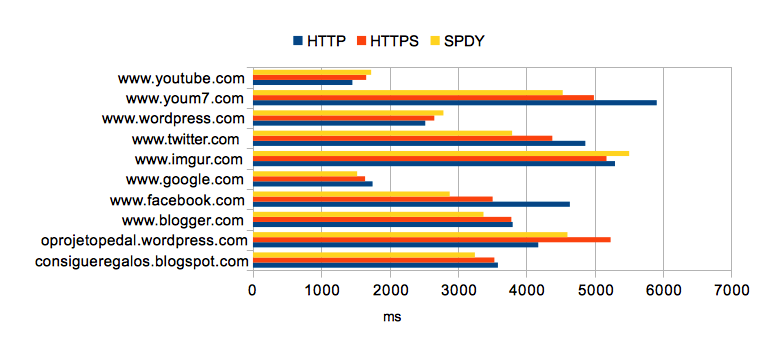
\includegraphics[scale=0.83]{exp2_1}
	\caption{\small onContentLoad}
	\label{graf7}
\end{figure*}

Por otra parte, este porcentaje frente a \textsc{https}, tambi'en es favorable en vistas de un posible HTTP 2.0 \cite{http2} que necesite ser encriptado obligatoriamente \cite{art1http2} \cite{art2http2} \cite{art3http2}. Ver Figuras \ref{graf7}, \ref{graf8} y \ref{graf9}.

\begin{figure}[h]
  	\centering
	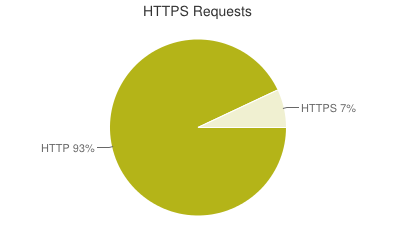
\includegraphics[scale=0.53]{httpvshttps}
	\caption{\small Porcentajes de utilizaci'on de los protocolos HTTP y HTTPS.}
	\label{httpvsthhps}
\end{figure}

\textsc{spdy} presenta resultados desfavorables en sitios con grandes contenidos, aquellos que necesitan de mucho tiempo para completar las peticiones, son proclives a tener p'erdidas de paquetes que necesiten de retransmitir el mensaje. Este tiempo que toma retransmitir todo el mensaje completo, hace que disminuya su rendimiento en la situaci'on mencionada anteriormente.

\section{Conclusiones}

\textsc{spdy} propone las bases para el futuro \textsc{http 2.0}, ofrece nuevas caracter'isticas que pueden ser aprovechadas y mejora la performance en ciertos casos. El protocolo es fuerte en condiciones en las que se presentan enlaces con Velocidades Bajas y con cierto Retardo, en condiciones favorables, el protocolo puede presentar inconvenientes por cuestiones de p'erdida de paquetes y retransmisi'on. Por otro lado, cabe destacar que, todas las t'ecnicas utilizadas para incrementar la performance\footnote{Css sprites, domain sharding, combinaciones de archivos de javascript, combinaci'on de archivos css, recursos as'incronos, etc.} no son necesarias para el buen funcionamiento del protocolo. El mejor escenario para \textsc{spdy} es el sitio con las caracter'isticas de \emph{worldflags}, es decir, con todos o la mayor'ia de los recursos en el mismo dominio, lo que aprovecha al m'aximo la multiplexaci'on de streams de datos.

\section{Trabajos Futuros}

A futuro una de las pruebas a realizar ser'ia, utilizando la suite de prueba del Experimento 1, ejecutar los tests pero con otros servidores que soporten SPDY, tales como \emph{Jetty Web Server}\footnote{http://wiki.eclipse.org/Jetty/Feature/SPDY}, \emph{Python implementation of a SPDY server}\footnote{http://github.com/mnot/nbhttp/tree/spdy}, \emph{Ruby SPDY}\footnote{https://github.com/igrigorik/spdy} o \emph{node.js SPDY}\footnote{https://github.com/indutny/node-spdy}. Para poder medir la performance de \textsc{spdy} en diferentes implementaciones del protocolo.

Otra herramienta apropiada para realizar mediciones es Selenium \cite{selenium}, con ella, se pueden automatizar diferentes interacciones con los sitios utilizando un navegador web. Si bien estos tests concluyen que \textsc{spdy} mejora la performance de la carga de un sitio, las caracter'isticas del protocolo se desempe'nan al m'aximo cuando el usuario se encuentra navegando el sitio. Con esta herramienta se podr'ia medir como se comporta \textsc{spdy} en una utilizaci'on cuasi real.

\begin{figure}[h]
  	\centering
	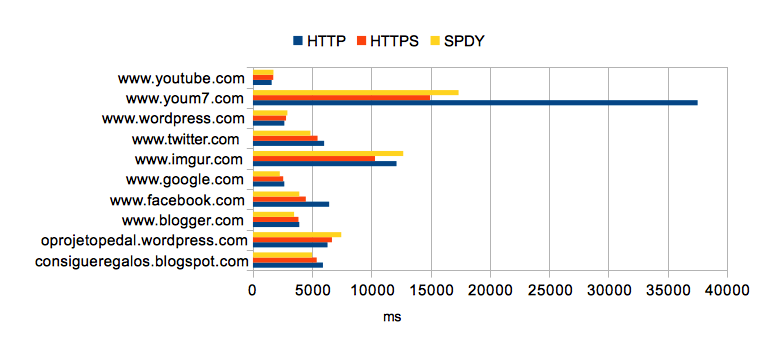
\includegraphics[scale=0.83]{exp2_2}
	\caption{\small onLoad}
	\label{graf8}
\end{figure}

\begin{figure}[h]
  	\centering
	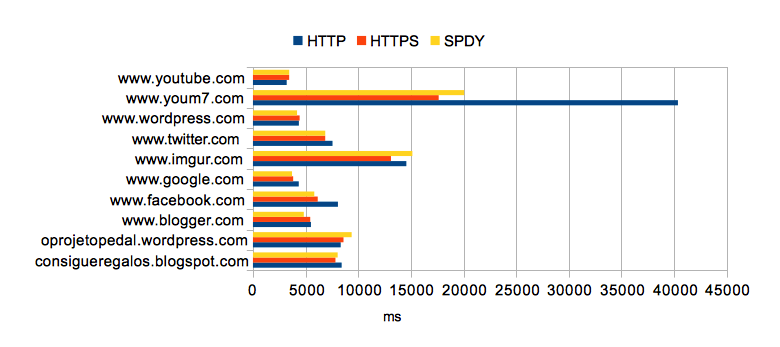
\includegraphics[scale=0.83]{exp2_3}
	\caption{\small ToW}
	\label{graf9}
\end{figure}

\onecolumn

\nocite{*}
\bibliography{bibliography}

\end{document}